\documentclass[en]{../../../../../../eplexam}

\usepackage{../../../../../../eplunits}
\usepackage[american]{circuitikz}

\hypertitle{powerelec}{7}{ELEC}{2660}{2016}{Janvier}{All}
{Louis Devillez}
{Marc Bekemans}

\section{Commenter ce slide /3}

\begin{figure}[H]
	\centering
	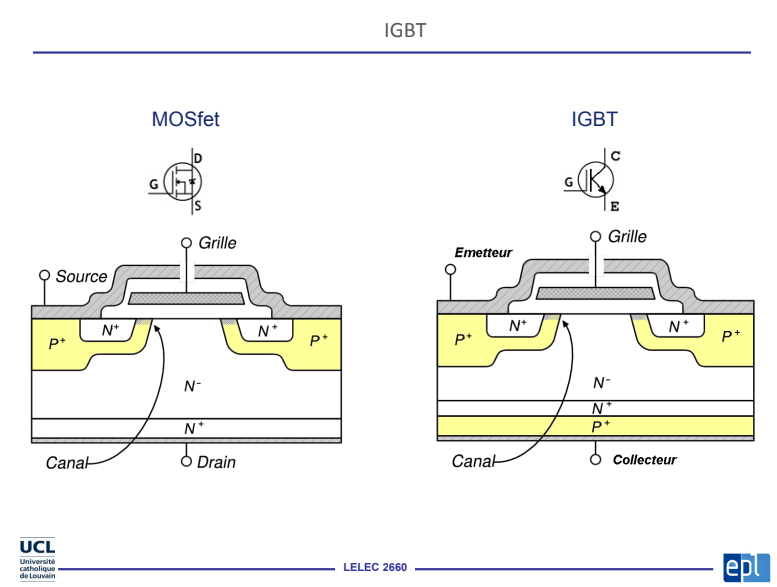
\includegraphics[width=0.65\textwidth]{Q1.png}
\end{figure}

\nosolution

\section{Commenter ce slide /3}

\begin{figure}[H]
	\centering
	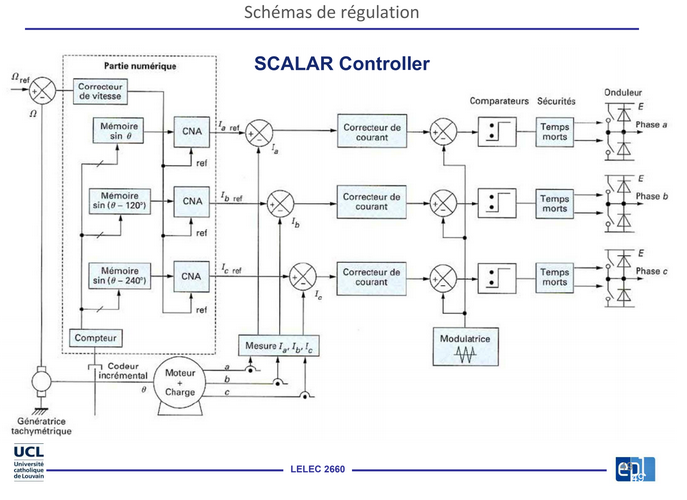
\includegraphics[width=0.65\textwidth]{Q2.png}
\end{figure}

\nosolution

\section{Série de questions à réponses courtes /8}

\begin{itemize}
	\item Quelle impédance caractéristique choisiriez vous pour réaliser le filtre d'entrée d'un convertisseur de \SI{50}{\watt} ($V_{out} = \SI{10}{\volt}$, $V_{in} = \SI{30}{\volt}$).
	\item Un thyristor, lorsqu'il n'est pas activé, peut bloquer des tensions positives et négatives. Vrai ou Faux ?
	\item Que vaut la puissance échangée entre deux sources de tension sinusoïdales reliées par une inductance de \SI{1}{\milli\henry} et déphasées de \SI{30}{\degree} ($V_a = \SI{300}{\volt}$ effectif, $V_b = \SI{400}{\volt}$ effectif).
	\item Quelle est la relation $I_{out}/I_{in}$ d'un convertisseur buck-boost ?
	\item Quelle est la tension DC obtenue par un redressement triphasé sans filtrage de la tension présente sur une prise de courant domestique (tension phase neutre de $\SI{220}{\volt}$).
	\item Un redresseur à thyristors permet de redresser de la tension DC vers AC. Vrai ou Faux ?
	\item Dans le cas du peak current control, le rapport cyclique est limité par la puissance de sortie. Vrai ou Faux ?
	\item Dans un onduleur triphasé alimenté en \SI{90}{\volt} DC, la tension instantanée max entre une phase et le point neutre (point étoile des 3 charges équilibrées) vaut:
	\subitem \SI{90}{\volt}
	\subitem \SI{45}{\volt}
	\subitem \SI{66}{\volt}
	\subitem \SI{33}{\volt}
\end{itemize}

\begin{solution}
\begin{itemize}
	\item $$P_{in} = P_{out}$$
	$$R_{load} \frac{V_{out}^2}{P} = \SI{2}{\ohm}$$
	$$||Z_N|| = \frac{R}{\theta^2} = \SI{18}{\ohm} << ||Z_0|| = \SI{1.8}{\ohm}$$
	\item Vrai
	\item $$P_1 = \frac{U_1U_2}{\omega L}\sin(\alpha) = \frac{400*300}{2\pi*50*10^{-3}}\sin(\alpha) = \SI{191}{\kilo\watt}$$
	\item 
	$$P = V_{in} I_{in} = V_{out} I_{out} \Rightarrow \frac{V_{out}}{V_{in}} = \frac{I_{in}}{I_{in}}$$
	$$V_{out} = \frac{-D}{1-D} V_{in}$$
	$$I_{out} = -\frac{1-D}{D} I_{in}$$
	\item $$V = \frac{3\sqrt{3}\sqrt{2}V_{rms}}{\pi} = \SI{514}{\volt}$$
	\item Faux
	\item Faux
	\item $V_{AN} = \frac{2}{3}V_{DC}$
\end{itemize}	
\end{solution}

\section{Expliquez, de façon détaillée, le fonctionnement d'un convertisseur flyback. Schéma, formes d'onde et explications /8}

\nosolution

\section{Soit un convertisseur boost présentant les caractéristiques suivantes: /12}
\begin{itemize}
	\item $V_{in} \in \left[\SI{50}{\volt}, \SI{90}{\volt}\right]$
	\item $V_{out} = \SI{100}{\volt}$
	\item $P_{out} = \SI{100}{\watt}$
\end{itemize}

\subsection{Quelles hypothèse pouvez vous faire sur les composants afin de pouvoir calculer le rendement ? /3}

\begin{solution}
	\item $V_{out}$ est parfaitement régulé.
	\item Uniquement perte par conduction
	\subitem Dans la diode $V_f = \SI{0.7}{\volt}$ et $R_{d} = \SI{0.02}{\ohm}$
	\subitem Dans l'inductance $R_l =\SI{0.2}{\ohm}$
	\subitem Dans le transistor $R_t = \SI{0.08}{\volt}$
	\item Les résistances n'influencent pas le fonctionnement du convertisseur mais ne sont que des pertes.
	\item La valeur rms des courant sera approximée par la valeur moyenne
\end{solution}

\subsection{Calculer tle rendement en fonction de $V_{in}$ (et des valeurs choisies au point précédent). /5}

\begin{solution}
	\begin{center}
		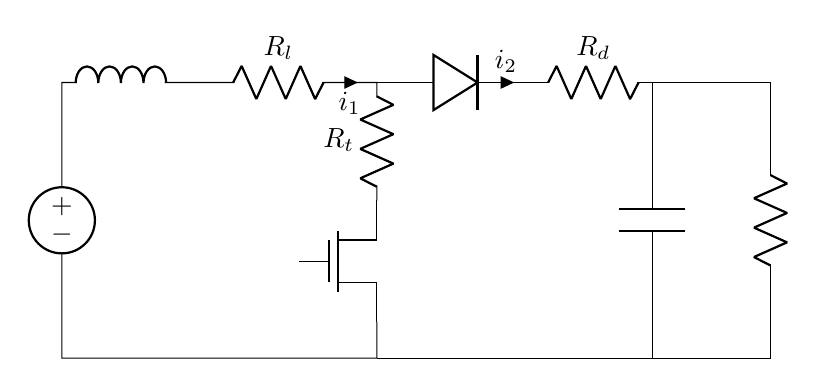
\begin{tikzpicture}
			\draw (0,0) node[nmos](nmos){};
			\draw (nmos.D) to[R,l=$R_t$] ++ (0,1.5) to[R,l_=$R_l$,i<=$i_1$] ++ (-2.5,0) to[L,mirror] ++ (-1.5,0) to[V] ++ (0,-3.5) -- ++(4,0) -- (nmos.S);
			\draw (nmos.D) ++ (0,1.5) to[D,i>=$i_2$] ++(2,0) to[R,l=$R_d$] ++(1.5,0) to[C] ++(0,-3.5) -- ++ (-3.5,0);
			\draw (nmos.D) ++ (3.5,1.5) -- ++ (1.5,0) to[R] ++(0,-3.5) -- ++(-1.5,0);
		\end{tikzpicture}
		
		$$\nu = \frac{P_{out}}{P_{out} + P_t + P_l + P_t}$$
		$$P_t = R_t * (i_{1,rms} - i_{2,rms})^2$$
		$$P_l = R_l *i_{1,rms}^2$$
		$$P_d = R_d * i_{2,rms}^2$$
		$$i_{ch} = \SI{1}{\ampere}$$
		$$i_{1,avg} = \frac{i_{ch}}{1 - \theta}$$
		$$i_{2,avg} = i_{ch}$$
		$$i_{1,avg} - i_{2,avg} = \frac{\theta i_{ch}}{1-\theta}$$
		$$\nu=\cfrac{100}{100+i_{ch} *\left(V_D + i_{ch}\left(R_t\frac{\theta}{1-\theta} + R_l\frac{1}{1-\theta} + R_d\right)\right)}$$
	\end{center}
\end{solution}


\subsection{Sur base de la formule trouvée, calculez le rendement pour $V_{in,min}$ et $V_{in,max}$ /4}

\begin{solution}
	$\theta_{min} = 0.5$ et $\theta_{max} = 0.1$
	$$\nu_{min} = 98.81\%$$
	$$\nu_{max} = 99.05\%$$
\end{solution}

\section{Déterminez le circuit dual du convertisseur ci-dessous. /4}
\begin{center}
	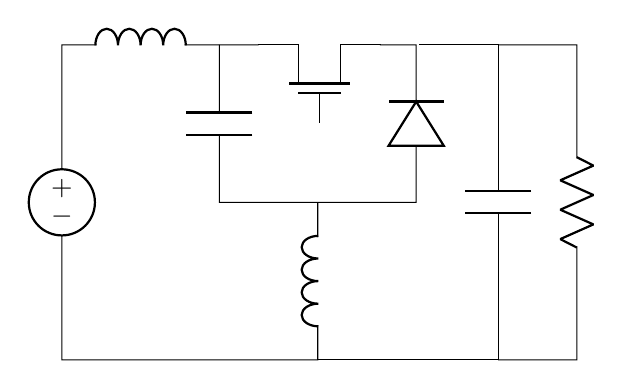
\begin{tikzpicture}
	\draw (0,0) node[nmos, rotate=90](nmos){};
	\draw (nmos.D) -- ++ (-0.5,0) to[C] ++ (0,-2) -- ++ (2.5,0) to[D] ++ (0,2) -- (nmos.S);in
	\draw (nmos.D) ++ (-0.5,0) to[L, mirror] ++(-2,0) to[V] ++ (0,-4) -- ++ (3.25,0) to[L] ++ (0,2);
	\draw (nmos.S) ++ (0.5,0) -- ++ (1,0) to[C] ++(0,-4) -- ++ (-2.3,0);
	\draw (nmos.S) ++ (1.5,0) -- ++ (1,0) to[R] ++ (0,-4) -- ++ (-1,0);
	\end{tikzpicture}
\end{center}

Bonus: Trouver le rapport $V/V_g$ de ce circuit.
\begin{solution}
	\begin{center}
		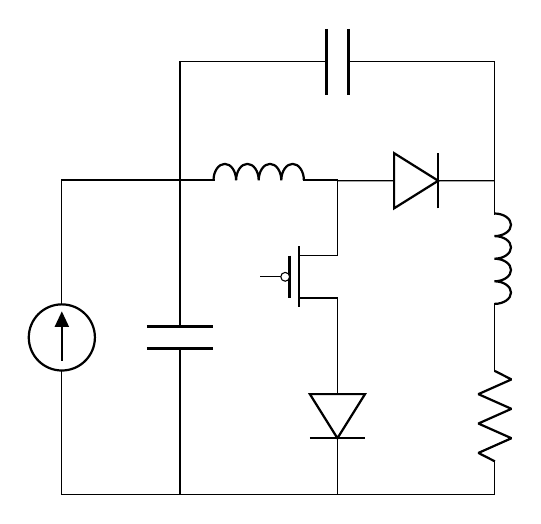
\begin{tikzpicture}
			\draw (0,0) node[pmos,emptycircle](pmos){};
			\draw (pmos.D) to[D] ++ (0,-2) -- ++ (-2,0) to [C] ++ (0,4) to[L] ++ (2,0) -- (pmos.S);
			\draw (pmos.D) ++ (-2,-2) -- ++ (-1.5,0) to[I] ++ (0,4) -- ++(1.5,0) -- ++ (0,1.5) to[C] ++ (4,0) -- ++ (0,-1.5) to[L] ++ (0,-2) to[R] ++ (0,-2) -- ++ (-2,0);
			\draw (pmos.S) ++ (0,0.45) to[D] ++ (2,0);
		\end{tikzpicture}
	\end{center}

Bonus: $V = \theta V_g$ (comme un buck)
\end{solution}
\end{document}
